\startchapter{Evaluation of The Gem Cutter Environment}
\label{chapter:Exp}

\begin{flushright}
\textit{...a scientist must also be absolutely like a child.  If he sees a thing, he must say that he sees it, whether it was what he thought he was going to see or not.  See first, think later, then test.  But always see first.  Otherwise you will only see what you were expecting.}
\\
Douglas Adams \cite{Adams84} \\
\end{flushright}

\section{The Cognitive Dimensions Framework}
\label{chapter:problemSec:cgframework}

\begin{flushright}
\textit{Every notation highlights some kinds of information at the expense of obscuring other kinds.}
\\
Thomas R. G. Green and Marian Petre \cite{green96} \\
\end{flushright}

One of the challenges faced in evaluating a programming environment is that programming is such a \textit{subjective}
task.  Different programmers have different preferences, and value certain features over others.  While one
programmer may find one aspect of the environment very useful, another may find that aspect counterintuitive.  
Programmers are famous for being extremely opinionated about the tools and environments they use, developing almost
dogmatic devotion to one approach at the expense of others.  It can be difficult to find a formal method to
use to discuss the merits of one language design over another that can be agreed upon.

When computer scientists and software engineers try to evaluate the usability of a system, they turn
to human computer interaction (HCI) principles to do so.  However, as pointed out in \cite{green96}, this is 
problematic for the evaluation of programming environments as typically HCI tends to focus on interactive situations
rather than notational design.  That is, HCI tends to focus more on ``micro-tasks'' and the finished product, rather
than the processes and activities which produce that task.  As an example, in evaluating a programming environment it is less important
to know that the ``compile'' option is easy to find than it is to know that the environment does not allow for new 
abstractions to be created.  Moreover, programmers are not HCI experts, and
vice-versa.  Thus while the vocabulary of HCI may be second nature to those in the field, it is less so for the
average computer programmer or software engineer.  Similarly, it is not uncommon for programmers to use terminology
that is unfamiliar to those who are not software developers.  For our purposes, we shall use the ``cognitive dimensions 
framework'' outlined by Green in \cite{green96} for evaluating differing visual programming environments.  

In this section we will outline the cognitive dimensions framework, giving an overview of the various dimensions of the framework, as well as recap some of the ways in which it has been applied to other environments.

\subsection{Outline of the Cognitive Dimensions Framework}
\label{cgframeoutline}

The Cognitive Dimensions Framework consists of 13 different ``dimensions'' to easily evaluate and critically examine a programming
environment.  The purpose of the framework is to provide a set of 
dimensions which capture much of the psychology and HCI of programming, and give a vocabulary which VPL
designers and users can use to examine different visual programming environments.  It is less of a framework
for stating that ``language X is better than language Y'', but more for statements like ``language X can have
better Y by changing Z'' (where Y is one dimension of the framework, and Z is some aspect of the VPE that
impacts Y).  Furthermore, the language used in the framework is more accessible to the average software developer, 
not requiring one to be an HCI expert to use it.

One very important aspect of the framework is that (not surprisingly) different dimensions can represent trade-offs.  In fact, 
this is intentional --- there are always trade-offs in designing any system of moderate complexity, and until there is a 
vocabulary for discussing those trade-offs it is difficult to reason about how one can improve the initial design.  The cognitive 
dimensions framework is intended as being able to fill this void, allowing designers to coherently and critically examine 
and \textit{converse} about their designs so that they may find the best compromise given the objective(s) of the system 
being designed.  As Green himself puts it ``Like other forms of engineering, design is a matter of compromise'' \cite{green96}.

Below is a recap of the listing of the thirteen dimensions of the Cognitive Dimensions Framework described by Green in \cite{green96}. 

\begin{itemize}
	\item Abstraction Gradient - What are the minimum and maximum levels of abstraction?
	\item Closeness of Mapping - What programming ``games''	need to be learned?
	\item Consistency - When some of the language has been learned, how much of the remaining parts of the language can be inferred?
	\item Diffuseness - How many symbols or graphic entities are required to express a meaning?
	\item Error-proneness - Does the design of the notation induce ``careless mistakes''?
	\item Hard Mental Operations - Are there places where the user needs to resort to fingers or penciled annotation to keep track of what's happening?
	\item Hidden Dependencies - Is every dependency overtly indicated in both directions? Is the indication perceptual or only symbolic?
	\item Premature Commitment - Do programmers have to make decisions before they have the information they need?
	\item Progressive Evaluation - Can a partially-complete program be executed to obtain feedback on ``How am I doing?''
	\item Role-expressiveness - Can the reader see how each component of a program relates to the whole?
	\item Secondary notation - Can programmers use layout, colour, or other cues to convey extra meaning, above and beyond the `official' semantics of the language?
	\item Viscosity - How much effort is required to perform a single change?
	\item Visibility - Is every part of the code simultaneously visible (assuming a large enough display), or is it possible to juxtapose any two parts side-by-side at will?
\end{itemize}

A more detailed description of each is given in the sections that follow.

\subsubsection{Abstraction Gradient}
\label{absgradientoutline}

Green describes the Abstraction Gradient as ``What are the minimum and maximum levels of abstraction?  Can 
fragments be encapsulated?''  Furthermore, Green classifies languages based upon three categories: abstraction-hating, 
abstraction-tolerant, or abstraction-hungry depending upon the languages minimum starting level of abstraction and their 
readiness or desire to accept further abstraction.

That is, this dimension asks the questions: how much needs to be constructed and learned in order to begin making the programming
environment perform a task?  And how easy is it to add new abstractions?  

The example Green gives of an abstraction-hating formalism is that of flowcharts, as they only allow decision boxes 
and action boxes.  There is no way to ``add'' additional constructs or group related ideas within a flowchart.  While they 
have a low minimum level of abstraction (there is not much to learn to begin using them), they have no readiness to accept
further abstractions.  Turing 
machines would be another example of a notation which is abstraction hating --- each instruction can only have a current 
state, current symbol, next state, next symbol, and a direction to move on the tape.

The classic example of an abstraction-tolerant language would be C, as it has a higher minimum level of abstraction (one must
learn some of the various keywords in the language, as well as how to write a \code{main()} routine for example), and it allows
for new abstractions of various kinds to be created (for example, one can create new types with \code{typedef} and \code{struct}).

The example Green gives of an abstraction-hungry language is Smalltalk, as it has a high starting level of abstraction, 
and requires one to modify the class hierarchy in order to create new programs.  That is, every program written in the
language \textbf{requires} the introduction of new abstractions.

From the perspective of learning to program, it has been shown that oftentimes
students new to computer programming struggle with languages which force one to learn and master several 
abstractions at once, giving them ``a `rubber hamburger' which has to be swallowed because it cannot be chewed''\cite{green96}.
As such it is difficult to find the right balance here, requiring too many abstractions to be learned can negatively
impact learning, but having limited abstraction mechanisms can make programs difficult to modify (see the section on Viscosity
later).  Green seems to indicate that abstraction-tolerant languages are the best fit for learning environments, but admits
that more research needs to be done in this area.

\subsubsection{Closeness of Mapping}
\label{closenessoutline}

One could argue that programming is all about problem solving.  Put another way, given a problem expressed in one particular domain (the problem domain) the role of the programmer is to come up with a mapping of this problem into the domain of the programming environment in use (the program domain).  Closeness of mapping tries to measure the gap between the problem domain and the program domain.  That is, how much extra ``administrative stuff'' does the environment impose upon the programmer in order to translate a solution to a problem into something that can be executed in the programming environment?  Green refers to this ``administrative stuff'' as ``programming games'', or the little language/environment-specific idiosyncrasies that are imposed upon the programmer.  The classic example of a programming game which is imposed on many first year computer science students is the \code{public static void main (String [] args)} method signature that must appear in any Java program.  This line is (typically) completely absent from the problem domain, yet is a required artifact that students must produce in order to produce a solution to any problem given to them by their instructors when Java is the language of choice\footnote{Assuming a development environment which consists of a plain text editor and the command-line based JDK from Sun}.

Closeness of Mapping also is to a lesser degree a measure of what the environment provides in terms of standard libraries and constructs.  If a language provides a great deal of standard libraries, then intuitively it would seem that there would be less work for the programmer to do to create the mapping from problem domain to program domain.  Related to this is the notion of whether or not the language allows constructs to be built that improve the Closeness of Mapping.  That is, if functionality is not provided in the way of standard libraries, is it possible for one to add their own to better bridge the gap between
problem and program domain.

Traditionally (and not surprisingly), domain-specific languages tend to score very well in this regard \emph{when the problem lies within the target domain that the language was designed for}.  It is less clear as to how well these languages score when attempting general problems that fall outside of that targeted domain.

\subsubsection{Consistency}
\label{consistencyoutline}

Consistency tries to measure how easy it is to infer the remaining parts of the language once one has learned part of the language.  Put another way, consistency assesses whether or not ``similar semantics are expressed in similar syntactic forms'' \cite{green98}. Green states consistency as a form of ``guessability'': ``when a person knows some of the language structure, how much of the rest can be successfully guessed?''\cite{green96}  An example that has been given for a way in which a language suffers from consistency problems is Pascal and its handling of reals and integers versus boolean variables.  In Pascal, one can read and write to reals and integers, but boolean variables may only be read from even though syntactically booleans are essentially used and treated in the same way as other variables.

Another more modern example would be Java and its String data type.  Strictly speaking, \code{String}s are object types in Java, but can be treated in much the same way as primitive data types (such as \code{int}s or \code{boolean}s).  For example, one can use the concatenation operator to combine two strings together in infix notation as seen in \pref{prog:javainfix}.  This is the only time in which object types may be used in this ``operator overloaded'' way, all other object types must resort to method calls (as seen in \pref{prog:javamethod}).  ``Special cases'' such as this can greatly hurt the consistency of a language and make them harder to learn.

\begin{program}
\begin{verbatim}
String s1 = "Hello";
String s2 = " World";
String s3 = s1 + s2;  // create "Hello World" 
\end{verbatim}
\caption{Concatenating Two Java Strings Using an Operator in Infix Notation}
\label{prog:javainfix}
\end{program}

\begin{program}
\begin{verbatim}
String s1 = "Hello";
String s2 = " World";
String s3 = s1.concat (s2); // create "Hello World" 
\end{verbatim}
\caption{Concatenating Two Java Strings Using Method Calls}
\label{prog:javamethod}
\end{program}

Typically visual languages tend to score well in consistency, largely due to a simpler syntax.  Many textual-based languages have struggled in regards to consistency as most ``real-world'' textual languages have grammars of substantial size, and generally speaking the larger the grammar, the more complex the syntax (and thus the more likely there will be inconsistencies that arise).
 
Additionally, as noted by Kelso an issue related to consistency is that of library regularity \cite{Kelso02}.  For example, Haskell generally keeps naming and argument ordering in libraries in regular order (thus scoring well in terms of consistency).  C libraries however tend to not score so well, largely due to the fact that they have been developed over a long period of time by a large number of authors\footnote{As well, it could be argued that the fact that all functions in C reside in the same namespace negatively impacts consistency as well as it means that library designers must come up with their own unique naming schemes for functions to avoid naming conflicts.}.

It has also been noted that consistency can be viewed from two different perspectives: the learner and the designer \cite{Reisner93}. Ideally these two perspectives should be the same, but in practice they often are not.  The distinction in Java between object types and primitive types is an example of this.  From the designers perspective this is perfectly consistent -- there are two fundamental categories of data types, and within the Java Virtual Machine (JVM) they are handled completely differently and separately.  From a learner's perspective however, this distinction can create confusion.  From a learner (or user of the language) it is all just data so the distinction is not as apparent and, for many new to the language, seems rather arbitrary.

At any rate, given that the Cognitive Dimensions framework was designed by Green to be used by designers of a language one might think that his intention was that consistency was to be applied from the designers perspective, however this is not explicitly stated.  From our perspective as evaluators of a VPE from a pedagogical standpoint we are however more interested in the learners perspective, and our application of this dimension in evaluating the Gem Cutter will reflect this.

\subsubsection{Diffuseness}
\label{diffusenessoutline}

Diffuseness is also sometimes referred to as terseness.  That is, it tries to measure how many symbols (or graphic entities in the case of a VPE) are required to express a meaning.  This is, of course, a trade off -- if a language is too terse it can be hard to read, but if a language is too verbose it becomes difficult to ``keep it all in your head'' at once.

Traditionally functional languages have been quite terse, and scored well in that regard\footnote{Some even criticize functional languages for being \emph{too} terse, further illustrating that this dimension represents a trade-off.}.  Visual languages also tend to require a small number of syntactic elements to express a meaning, so one would think that a visual functional programming environment would be the most terse of all environments, and Kelso found this to be true of his VFPE \cite{Kelso02}.

Measuring diffuseness/terseness is done by counting the number of syntactic lexemes that comprise a program.  To give a meaningful comparison, Green uses a sample yardstick problem taken from \cite{curtis89} that he calls the ``rocket trajectory problem'' which he summarizes as:

\begin{quotation}
The rocket program computes the vertical and horizontal trajectory of a rocket on which the only forces acting are its thrust and gravity.  At time zero the rocket stands stationary and vertical on level ground, with a mass of $10^4$ pounds.  Its engine develops a thrust of $4\cdot10^5$ foot-pounds, using up a mass of 50 pounds of fuel per second, until the fuel is exhausted after 100 seconds.  It rises vertically for 10 seconds after which it adopts and retains an angle of 0.3941 radians (22.5 degrees) to the vertical.  The downwards acceleration of gravity is $32 feet/sec^2$ \cite{green96}.\label{rocketproblem}
\end{quotation}

%in \fref{fig:rocketTrajectoryProblem}.  
%\begin{figure}
%The rocket program computes the vertical and horizontal trajectory of a rocket on which the only forces acting are its thrust and gravity.  At time zero the rocket stands stationary and vertical on level ground, with a mass of $10^4$ pounds.  Its engine develops a thrust of $4\cdot10^5$ foot-pounds, using up a mass of 50 pounds of fuel per second, until the fuel is exhausted after 100 seconds.  It rises vertically for 10 seconds after which it adopts and retains an angle of 0.3941 radians (22.5 degrees) to the vertical.  The downwards acceleration of gravity is $32 feet/sec^2$.\cite{green96}
%  \caption{The Rocket Trajectory Problem}
%  \label{fig:rocketTrajectoryProblem}
%\end{figure}

He then goes on to give solutions to the problem in each of the environments he looked at, and Kelso did the same for Haskell and his VFPE.  The unfortunate flaw in this approach is that it does not account for individual skill or familiarity with a language -- the more familiar one is with a programming environment, the more likely it will be that one can use the ``right'' constructs and thus produce a solution which is the most terse.  Conversely, if one is unfamiliar with an environment\footnote{And particularly if the environment suffers from poor consistency} one will likely try to use a subset of the full set of constructs available, and end up producing a solution which is overly ``cluttered''.

As well, as noted by Kelso in \cite{Kelso02} it can be difficult to measure diffuseness in visual environments which have dynamic layout schemes.  Oftentimes visual environments allow one to ``collapse'' code blocks into single elements.  Or as Kelso puts it: ``The level of diffuseness can in effect be dynamically traded off against the level of detail''.

\subsubsection{Error-Proneness}
\label{errorpronenessoutline}

The fundamental question that the error-proneness dimension tries to answer is ``does the design of the notation induce `careless mistakes'?''  Green draws a distinction between `mistakes' and `slips', where the former refers to the parts of program design which are deeply difficult irregardless of the notation\footnote{For example, design issues such as how to decompose a larger problem into smaller ones would be an example of a ``deeply difficult'' design problem.}, and the latter refers to those errors that one did not mean to do, where you knew better, but still somehow made a simple little ``slip-up''.  Error-proneness tries to measure whether or not the notation itself oftentimes leads to or encourages these ``slips''.

An example from the world of textual languages is the use of textual identifiers, particularly in languages which are case-sensitive.  It is very easy to accidentally misspell an identifier in languages which do not require identifiers to be declared before they are used, which can lead to subtle and difficult to debug errors in the program.  The paired-delimiter system (braces in C/C++/Java, parenthesis in languages such as Lisp and Scheme, or the begin/end pair in languages like Pascal) can also lead to trivial errors which cause the code to fail to compile.  Note that all of these are \emph{syntax} errors which are all but avoided in visual programming languages.  Thus, not surprisingly visual environments tend to avoid some of these common ``slips'', however, it would not be fair to say that visual languages are inherently less error-prone than textual languages.

\begin{comment}
Languages such as Pascal which use semicolons as separators rather than statement terminators can cause confusion as well, as often times novices will write: 

\code{if A then B; else C;}

rather than 

\code{if A then B else C;}

The functional language SML has a similar issue in regards to its ``let expression'' syntax.  FIXME - perhaps reference SML reference manual with explanation of how val bindings in lets do not need to end with semicolons.
\end{comment}

Kelso in \cite{Kelso02} also notes that issues related to data types can play a role here.  That is, languages which have strong type checks that are enforced throughout a program will likely be less error-prone than languages which do not enforce such strong and rigorous type checking.

\subsubsection{Hard Mental Operations}
\label{hardmentalopsoutline}

A programmer must already juggle a number of different ideas and concepts while implementing the solution to a task.  What data structure should I use?  How efficient is this algorithm?  Can I access this piece of data within this context?  Ideally we would like our programming environments to reduce the cognitive load imposed upon the programmer.  That is, a programmer's job is hard enough, without having the tools in use add to the amount of things he or she must juggle.  This is where the hard mental operations dimension comes in.  Green defines a hard mental operation as having two properties:

\begin{enumerate}
	\item it must lie at the notational level, rather than the semantic level, as the dimension is trying to measure shortcomings in the programming environment, rather than discover meanings which are inherently difficult to express irregardless of the notation
	\item combining multiple hard mental operations vastly increases the difficulty
\end{enumerate}

As such, this allows him to outline a ``broad-brush'' test for hard mental operations by asking the following two questions: 

\begin{enumerate}
	\item if I fit two or three of these constructs together, does it get incomprehensible?
	\item is there a way in some other language of making it comprehensible? (Or is it just a really hard idea to grasp?)
\end{enumerate}

If the answer to both is yes, then we have a hard mental operation.  As an example application of this, consider the following declaration written in the C programming language:

\[
\code{int *(*(*(*b)())[10])();}
\]

This is taken from \cite{Giguere87}, and it is a declaration which declares a pointer to a function called b which returns a pointer to an array of 10 elements, each of which are pointers to functions which return pointers to ints.

If we examine ``functions as parameters in C'' as a construct, we would ask the question ``if I fit two or three function pointers together, does it get incomprehensible?''  It would appear that the answer to this is yes, a pointer to a function is difficult to mentally parse to begin with, but if we have pointers to functions of pointers to functions, they are even more difficult to decompose.  Next we ask the question ``is there a way in some other language of making function pointers comprehensible?''  Given that higher order functions are essentially functions as parameters, most any functional programming language provide support for this mechanism in a much simpler and easier to understand form.  Thus, it would appear that ``functions as parameters'' is an example of a hard mental operation in the C programming language.

Hard mental operations in particular is an important dimension for environments designed for learning, as presumably students learning a language already have to mentally process the new language or notation that they are learning, in addition to any fundamental ideas or concepts instructors are trying to convey.  Put another way: hard mental operations increase the cognitive load upon students, and this can have a negative impact upon learning.

\subsubsection{Hidden Dependencies}
\label{hiddendependenciesoutline}

A hidden dependency occurs when there is a relationship between two components such that one is dependent upon the other, and for which this dependency is not fully visible or apparent.  An example from the textual domain that is of particular interest to programmers working within the functional paradigm is that of the side effect.  If we have a subroutine \code{a()} which alters a global variable, this represents a hidden dependency between the variable and the function.  One of the hallmarks of the functional paradigm is the notion of referential transparency, whereby an expression can be replaced with its value without altering the meaning or semantics of the program as a whole, a definition which prohibits these sort of side effects.

Another common example includes the much maligned GOTO statement found in various programming languages.  This is due to the absence of a ``come-from'' which means that the effect of changes to code making heavily use of GOTOs can be difficult to predict.

A much more systemic example of a hidden dependency is the construct that virtually all programming languages make use of -- the named subroutine.  If \code{a()} calls \code{b()} which calls \code{c()}, a change to \code{c()} has implications for both \code{a()} and \code{b()}, though that relationship will likely not be apparent unless one examines the code of those routines.  Call graphs are commonly used to mitigate this concern.

\subsubsection{Premature Commitment}
\label{prematurecommitmentoutline}

The fundamental question to be asked in regards to this dimension is ``do programmers have to make decisions before they have all the information they need?''  Green explains premature commitment is akin to ``writing the contents list -� with page numbers �- before you write the book''\cite{green96}.  Premature commitment occurs when the following three criteria are met:

\begin{itemize}
	\item the notation contains many internal dependencies
	\item the medium/environment constrains the order of doing things
	\item the order is inappropriate
\end{itemize}

For example, consider the C function defined in \pref{prog:hypoCsub}.  In isolation, a source file containing only this code would not compile as there is an internal dependency between the \code{foo()} subroutine, and another routine called \code{bar()}.  The typical C programming environment constrains one from writing subroutines which depend on other subroutines until a definition of those subroutines are given\footnote{The common ``work-around'' for this is the stub routine, where the function prototype and an empty body (or a simple return statement for routines which have return types) is provided by the programmer, and ``filled-in'' later}.  Whether or not this constraint on the order of subroutine creation is appropriate or not shall be left for the reader to decide.

\begin{program}
\begin{verbatim}
int foo ()
{
    return bar() * 42;
} 
\end{verbatim}
\caption{A Hypothetical C subroutine}
\label{prog:hypoCsub}
\end{program}

Furthermore, Green provides a number of categories of premature commitment, outlined as:

\begin{itemize}
	\item Commitment to layout
	\item Commitment to connections
	\item Commitment to order of creation
	\item Commitment to choice of construct
\end{itemize}

\subsubsection{Progressive Evaluation}
\label{progressiveevaluationoutline}

This dimension tries to evaluate to what degree the environment in question allows one to evaluate a partially completed solution.  That is, environments which are strong from the perspective of progressive evaluation will allow evaluating partially complete programs with greater frequency.

As such, traditional text-based, compiled languages tend to score poorly in this dimension -- a Java program cannot be executed until it is compiled, and it cannot be compiled until it is a complete program.  Interpreted environments can do better, as they oftentimes allow one to enter individual expressions and evaluate them at any time\footnote{This is, in fact one of the arguments in favour of using Python as an introductory programming language, as the standard Python interpreter allows one to enter expressions and get immediate results}.  There are still limitations in that the expressions must be ``self-contained'', they cannot contain references to not yet identified values or functions for example.  However, this is more an issue of premature commitment than one of progressive evaluation.

This dimension is of particular importance to students new to programming, as it is recognized that novices need to evaluate their progress frequently to assess whether or not they are appropriately understanding the new concept or idea.

\subsubsection{Role-Expressiveness}
\label{roleexpressivenessoutline}

Role-expressiveness concerns the environments support to answer a user's query of ``what is this bit for?''.  That is, how easy is it for a user to see how various component parts of the program relate to the program as a whole.  Green identifies four specific items which relate to role-expressiveness:

\begin{itemize}
	\item meaningful identifiers
	\item well-structured modularity
	\item use of secondary notation (see below) to signal functionally-related groupings
	\item ``beacons'' which signify highly diagnostic code structures
\end{itemize}

For example, LabVIEW does not support identifiers of any kind, thereby increasing the difficulty of comprehending a given LabVIEW program.  Different languages have different levels of support for modularity as well.  For example, Java allows one to break up a program into classes, each of which contains methods.  This modularity improves the ability for one to understand (particularly larger) programs.  Code ``beacons'' are defined by Wiedenbeck as ``key features [in a program] which indicate the presence of a particular structure or operation'' and are identified as ``idiomatic or stereotypical elements in program code'' \cite{Wiedenbeck91}.  As an example, in looking at a sorting routine one typically expects to find some code which is responsible for swapping two elements that are incorrect order.  The ``swap'' beacon helps programmers to understand the sorting program as a whole.  It has been shown that recognition of beacons in code is strongly correlated to programmer experience.  A study done by Wiedenbeck found that while 79\% of experienced programmers recalled significantly more of the beacon lines in a program, only 14\% of novices could do the same \cite{Wiedenbeck91}.  Related to role-expressiveness, some languages encourage certain beacons to appear and some do not.  Using the same sorting example, the code in \pref{prog:haskellqs} shows the Quicksort routine written in the Haskell programming language.  Note that there is no ``swap'' beacon in this code.

\begin{program}
\begin{verbatim}
qsort []     = []
qsort (x:xs) = qsort (filter (< x) xs) ++ [x] ++ 
               qsort (filter (>= x) xs)
\end{verbatim}
\caption{Quicksort in the Haskell Programming Language\cite{haskellIntro}}
\label{prog:haskellqs}
\end{program}

Green also notes that role-expressiveness is one of the most difficult dimensions to clarify, largely due to a lack of ``studies on comparative comprehension of equivalent programs expressed in different notations'' \cite{green96}.

\subsubsection{Secondary Notation}
\label{secondarynotationoutline}

The dimension of secondary notation concerns how much extra information beyond the official syntax of a notation can be conveyed.  The classic example of secondary notation from the world of textual programming is the comment.  Comments have no bearing on the final program\footnote{And are often removed completely during the compilation process}, and are present solely for the purpose of providing extra information to other programmers examining the code.  Other examples include indentation, naming conventions, and grouping of related statements.

In the visual world, the analogues include things such as layout of graphical entities, the use of colour and/or shapes, or other cues to convey extra meaning.  For example, perhaps one construct may uniformly always be coloured a particular way.  For example, the Alice VPE makes extensive use of colour to convey extra information to the user.  In \fref{fig:aliceComp-a} we see that properties of an object\footnote{The object in question is the ``IceSkater'' object from the default Alice tutorial} are listed in rectangular boxes that are coloured yellow, whereas in \fref{fig:aliceComp-b} we see that methods of the same object are coloured a beige colour, and finally in \fref{fig:aliceComp-c} we see functions are coloured a violet colour. 

\begin{figure}[htp]
  \begin{center}
    \subfloat[Properties of an Object in Alice]{\label{fig:aliceComp-a}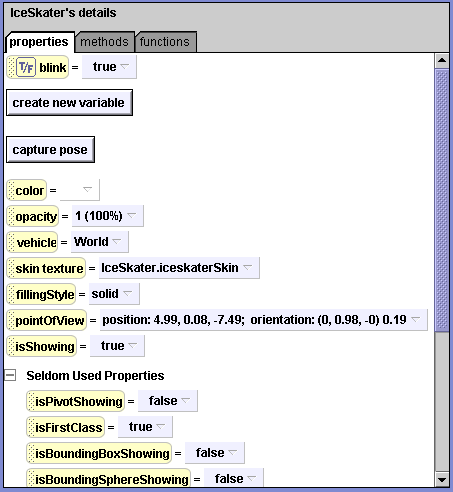
\includegraphics[scale=0.5]{Figures/aliceProp}} \\
    \subfloat[Methods of an Object in Alice]{\label{fig:aliceComp-b}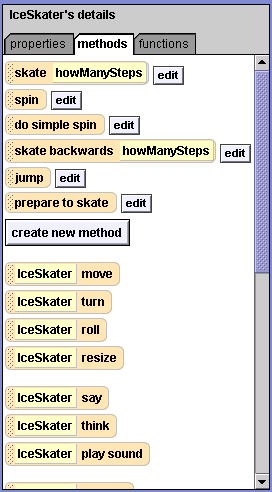
\includegraphics[scale=0.5]{Figures/aliceMeth}} \quad
    \subfloat[Functions of an Object in Alice]{\label{fig:aliceComp-c}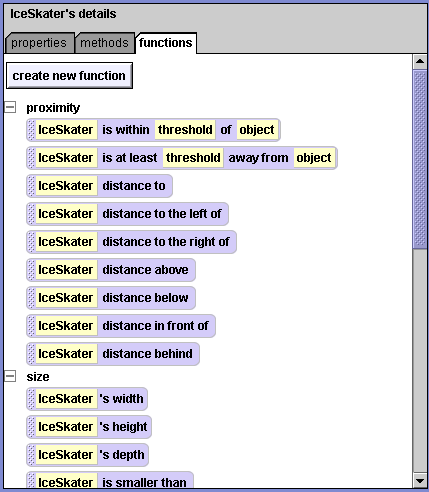
\includegraphics[scale=0.5]{Figures/aliceFunc}}
  \end{center}
  \caption{Components of the Alice Interface}
  \label{fig:aliceComp}
\end{figure}

Secondary notation can be related to visibility (see below), in that a secondary notation may be present, but if it is not readily apparent then its usefulness is somewhat diminished.  As well viscosity (see below) can impact secondary notation, as if a system is very viscous then changing the layout may be artificially difficult causing an aversion to changing the layout of a program after it has been initially constructed.  As well, if the structure is changed, then the secondary notation can go out of date and become a detriment to aiding understanding of a program.  Green also acknowledges that perhaps novices may benefit from a more constrained system in which secondary notation is minimized, but admits that this is pure conjecture and that more research needs to be done to confirm or deny this hypothesis \cite{green96}.

\subsubsection{Viscosity}
\label{viscosityoutline}

Viscosity measures resistance to change.  A system which is highly viscous is one where seemingly small changes require a relatively large amount of effort to undertake.  This can of course be dependent upon the specific change in question, but certainly some environments make changes more difficult than others.  Green identifies two particular types of viscosity:

\begin{itemize}
	\item Repetition viscosity, where one change implies that the same change will have to be made elsewhere a number of times
	\item Knock-on viscosity, where one change implies many other changes to the whole to restore consistency
\end{itemize}

An example of repetition viscosity would be changing the name of an identifier in a textual language as each use of the identifier will have to be changed to the new name.  An example of knock-on viscosity is changing the return type of a function, as this will require one to change all code which makes use of the return value of the function to make the program syntactically correct again.

Given how many software systems evolve over time viscosity is a rather important dimension.  Additionally from the perspective of students learning to program, oftentimes students will make mistakes early on and correct them after the fact.  If the system is highly viscous this can be problematic, as the effort to correct mistakes can become a deterring factor in a students motivation to produce a high quality solution rather than one that is ``good enough''.

Kelso notes that oftentimes VPE's suffer from viscosity problems due to the overhead of managing layout.  There is an overhead associated with laying out and rearranging components in a way that conveys extra meaning (aiding secondary notation), and without making the layout seem ``cluttered''.  He argues that this is an inherent problem in any VPE which requires manual layout and formation of links between components \cite{Kelso02}.  Additionally, an editor which enforces program correctness\footnote{Which many VPE's do given that one of the goals of a VPE is the removal of syntax errors} imposes an impediment on changing or rearranging components.

Viscosity can be related to premature commitment, as if one has to make a design decision too early it is probable that that choice will need to be revised.  If the system is highly viscous then those changes will be difficult to incorporate, whereas if it has low viscosity then the changes should be easy to implement.  That is, ideally a system which suffers from premature commitment should have low viscosity otherwise the problems related to premature commitment are amplified.

Given that the amount of time and effort to incorporate a change is dependent not only on the notation but also the specific change in question, viscosity has oftentimes been measured by implementing a small change to the rocket trajectory program\footnote{Described on page \pageref{rocketproblem}} to take account of air resistance, by exerting a drag proportional to the square of the velocity, and measuring the amount of time it takes to implement this change.  Because the goal of this test is to measure editing time and not the time taken to solve the problem, the test is conducted in two stages.  First a solution to the new problem is created, a screen capture of the new solution is taken, and then the original rocket program along with the screen capture of the extended version is provided and the time measured is that of how long it takes to turn the original into the new modified version.

\subsubsection{Visibility}
\label{visibilityoutline}

Visibility concerns ``whether required material is accessible without cognitive work; whether it is or can readily be made visible, whether it can readily be accessed in order to make it visible, or whether it can readily be identified in order to be accessed'' \cite{green96}.  Related to visibility is juxtaposability, the ability to view two or more components side-by-side.  For example, can a user display two subroutine designs simultaneously so as to be able to compare and contrast them?

Visibility is in some senses similar to hidden dependencies, but while hidden dependencies measure whether relationships are manifest whereas visibility is concerned with the number of steps needed to make a given item visible.

In general VPE's tend to suffer from visibility problem insomuch as there is only a limited amount of screen space available to display constructs, and typically a graphical notation tends to take up more visual space than a textual one.  While graphical displays have increased in size and resolution over time, this can still remain a problem inherent to visual representations.

\subsection{Application of the Cognitive Dimensions Framework to Other Environments}
\label{sec:prevAppCG}

In this section we will briefly recap the application of the Cognitive Dimensions framework to three different visual programming environments: Prograph, LabVIEW, and the VFPE from \cite{green96,Kelso02,green98,Green00}.

In terms of abstraction gradient, both Prograph and the VFPE were found to be abstraction tolerant.  Both allowed the introduction of new abstractions, however it was argued that the VFPE had a lower minimum level of abstraction as little needs to be learned to begin working with the environment.  LabVIEW however was found to be an abstraction hating language, as it provides no way of adding new abstractions past the ``bundle of wires'' construct.

As a domain specific language, LabVIEW has excellent closeness of mapping for problems in the electronics simulation domain, but outside of that domain there were difficulties expressed due to the fact common constructs required extra ``administrative stuff'' (such as looping requiring knowledge of the shift register to transfer values from the end of one iteration to the next).  The library support in LabVIEW reflected the domain specific nature of the language as well, limiting the positive closeness of mapping largely to the domain of electronics simulation and circuit design.  The VFPE and Prograph as general programming environments do not suffer from the same limitation.  In particular the library support of the VFPE was found to be somewhat weak compared to other environments used in industry, and as such more code was required to achieve similar results, thereby hurting the closeness of mapping from problem to program domain.  

VPE's in general have been found to score well in regards to consistency due to the simpler syntax.  No specific problems related to consistency were noted about LabVIEW, Prograph, or the VFPE.  Additionally, the VFPE standard library is based upon the Haskell standard library which when possible keeps argument naming and order consistent, thereby also improving this dimension in that environment.
 
In terms of diffuseness or terseness, VPE's have traditionally suffered due to the fact that graphical entities tend to consume more screen real estate than textual lexemes.  The sample rocket program mentioned on page \pageref{rocketproblem} was implemented in all three environments to measure this dimension.  The LabVIEW implementation consisted of 45 icons and 59 wires for a total of 104 graphical entities and fit easily onto a ``medium sized screen'' \cite{green96}.  The Prograph implementation occupied 11 windows, with a total of 52 icons and 79 connectors to give a total of 131 graphic entities, and would not fit onto a single screen.  Being a functional language, it is not particularly surprising that the VFPE was found to be quite terse and the sample implementation of the rocket program consisted of 98 graphic entities.  The counts for the VFPE did not include node-joining lines as they are semantically redundant and drawn by the environment, not the user.

In terms of error-proneness, most VPE's essentially eliminate typographical and syntax errors due to the constrained interface and all three environments were found to share this property.

Hard mental operations were discovered in LabVIEW and Prograph.  The difficulties in LabVIEW seemed to mostly arise due to the use of logic gates in conditionals, as users tried to ``trace'' through the connections between the gates.  This was somewhat surprising as the notation for logic gates is very well known.  Green speculated that perhaps this difficulty may be due to the fact that the notation evolved from a paper-based notation, where users can pencil in intermediate results as they trace through the various connections between gates.  Since LabVIEW does not provide a facility for this, users have to keep in their head the intermediate results of conditional expressions.  Difficulties in Prograph were noted surrounding control of loops.  In terms of the VFPE no specific hard mental operations were identified, however it is not clear if this is an indication of the absence of hard mental operations, or simply that none were noted. 

The box-and-wire representation used in many VPE's greatly helps to avoid hidden dependencies at the local level, as it makes the dependency between components visually explicit.  All three environments displayed this.  Past a local level however, Prograph in particular greatly suffers from issues related to hidden dependencies due to deep nesting and no overview of the nesting structure.  One can navigate down a call graph by clicking methods to open up a window for that method, but the reverse is not true.

In regards to premature commitment, it was also noted that VPE's using the box-and-wire representation tended to allow fewer constraints on the order of creation of code.  That is, none of the three visual environments surveyed were found to have any issues with respect to commitment to order of creation.  LabVIEW was found to have difficulty with commitment to layout, due to the fact that the environment was so viscous (changes after the fact were difficult to do).  Prograph had great problems in regards to commitment to connections, as avoiding the ``visual spaghetti'' of wires crossing over one another took a great deal of lookahead on the part of the user.  Again, viscosity was cited as a problem as if one chose a poor layout of components in a Prograph program which lead to overlapping wires, modifying it to improve the layout was difficult.  The VFPE was found to be very strong in terms of commitment to layout and commitment to connections as both are controlled by the environment.  The drawback to this is that secondary notation is negatively affected as layout cannot be used to convey extra meaning as would be the case in a more freeform layout scheme.  It was also noted by Kelso that any syntax-directed editor (such as the VFPE) will always suffer from problems related to premature construction commitment problems unless it allows easy relocation of code into temporary ``meaningless'' locations.

Both Prograph and the VFPE were found to have strong support for progressive evaluation as both allowed the ability execute program fragments as opposed to requiring entire complete programs before execution can take place.  Prograph in particular was quite strong in this regard as it allows program fragments to be executed which can even contain unfinished structures (the interpreter will execute up to the point where there is unfinished code).  The VFPE allows any expression can be evaluated so long as it is complete.  LabVIEW however required that a complete program must be constructed before any execution can take place.

LabVIEW was found to have significant problems in regards to role expressiveness, due to the absence of identifiers, poor secondary notation and ``beacons'' of code.  Secondary notation was somewhat aided by the extensive control over program layout as well as the ability to add comments to components and wires\footnote{But not groups of components}.  Viscosity is hurt by this however, as the overhead of rearranging components made small changes more costly.  Prograph programs contained identifiers to help role expressiveness, but this dimension also suffered from problems related to secondary notation, as the secondary notation in Prograph was found to be very limited.  Comments could be applied to primitives and methods, but not groups of objects.  Secondary notation is partially aided by the ability to control layout of components, however, this turns out to be diminished by the need to minimize wire crossings (which had a negative impact on viscosity).  Support for role-expressiveness in the VFPE was found to be aided by the ability to add as many or as few identifiers as one wishes.  Kelso also identified some common ``beacon'' structures that tended to arise in the VFPE such as compositional pipelines appearing as a vertical string of beads, and arithmetic expressions tending to form into pyramids.  There was however little support for secondary notation identified in the VFPE, short of the ability to add comments to any node (sub-expression), and even this was hurt by the lack of a visual indication of the presence of a comment.  The automatic layout of components was found to aid viscosity as it was identified that the freedom to arrange components imposed an overhead on any change to the program as one would have to rearrange the components, however, this came at the cost of secondary notation as layout could not be used to convey extra meaning.

In terms of Viscosity, the ``straw test'' of making the small change to the rocket program was done with each of the three environments, and took 508.3 seconds in LabVIEW, 193.6 seconds in Prograph, and 105 seconds in the VFPE.  Specifically, the LabVIEW version took so long due to the fact that connections had to be rebuilt when components were rearranged.  It was also noted that all three visual environments took significantly longer to incorporate the change than doing so in a traditional textual environment, as the same rocket trajectory program was implemented in Microsoft BASIC, and the ``straw test'' change took only 63.3 seconds.  Thus while visual environments tend to be rather terse (i.e. - have strong diffuseness), they also tend to suffer from viscosity problems.

LabVIEW was found to suffer from problems in regards to visibility and juxtaposibility, in particular the conditional was identified as being a significant problem.  In LabVIEW, a conditional can only display one branch of the conditional at any time, a clear violation of juxtaposibility.  The VFPE suffered from a similar problem with patterns in expressions.  With patterns in the VFPE, only one ``case'' can be displayed at any given time, there is no way to simultaneously display all cases of a pattern.  As well, oftentimes more complex expressions can be automatically laid out in a way that is impossible to view on a single screen, thereby making it impossible to juxtapose distant parts of the same expression.


\section{Applying the Cognitive Dimensions Framework to the Gem Cutter}

In this section we shall apply the Cognitive Dimensions framework developed by Green to the Gem Cutter VPE.

\subsection{Abstraction Gradient}

As described in \sref{cgframeoutline} the Abstraction Gradient dimension tries to measure how much needs to be constructed
and learned in order to begin making the programming environment perform a task, and additionally how easy is it to add new abstractions to the environment.

\subsubsection{Discussion of Dimension}

In regards to the Gem Cutter, much like the VFPE, as a functional language there is a relatively small set of constructs to master before making the environment perform a task.  As a base minimum, one only needs to be familiar with the notion of a function, and how a gem is a visual representation of that concept, along with the mechanics of how to connect gems together on the tabletop.  As one wishes to do more sophisticated tasks, introduction of the additional gem types\footnote{Such as collector/emitter pairs, value gems, code gems, and record gems} will be required, however, this is still a relatively low minimum level of abstraction.  This is a great strength of the Gem Cutter, particularly from the perspective of a student learning to program, as little needs to be learned and mastered before beginning to make the environment perform basic tasks.

The Gem Cutter like most programming languages, would be an example of an abstraction-tolerant language, though only barely.  The only mechanism for introducing new abstractions is the ability to define new gems and use those gems in other gem designs.  Aside from this basic abstraction mechanic there is little or no support for introducing new abstractions.  In particular the lack of ability to introduce new types as discussed in \sref{sec:gemCutterShortcomings} greatly hinders ones ability to introduce new abstractions to reduce the complexity of larger problems.  This is mitigated somewhat by the introduction of code gems which allow one to introduce CAL code snippets at any point into a gem design.  Since CAL is very much an abstraction-tolerant language fully supporting the ability to introduce and define new types, this allows a ``loophole'' where one can bring all the expressive power of CAL to the Gem Cutter.  However, code gems will only be useful to those who already understand the CAL language.  This would be roughly analogous to requiring users of Alice to write Java code to create new object types to use in their Alice programs, which would seem rather cumbersome.

\subsubsection{Remedies, Workarounds, And Trade-offs}

Green suggests that a possible remedy for problems related to the abstraction gradient of an environment is to introduce incremental abstractions.  This would be where the environment has a low starting abstraction barrier (ie - start with a low minimum level of abstraction where little needs to be learned to begin working with the environment), and to allow the introduction of new abstractions that will aid users later.  To a certain degree the Gem Cutter does this already, as there is a relatively low minimum level of abstraction as mentioned above, and one can learn about the other gem types as they progress with the environment.  What is missing are enhanced facilities for newer abstractions, most notably in regards to types.  The introduction of a mechanism for defining a new type in a visual way would help to alleviate this aspect much more than the current ``workaround'' of using code gems.

%------------------------------------------------------------------------------------------------

\subsection{Closeness of Mapping}

As described in \sref{cgframeoutline} the dimension of Closeness of Mapping tries to measure the gap between the problem domain and the program domain. 

\subsubsection{Discussion of Dimension}

In terms of ``programming games'', the Gem Cutter imposes relatively few upon the user.  As a visual functional language, the notation of the Gem Cutter is rather concise.  Sometimes gem designs can become ``cluttered'' with an excessive number of visual entities, but this is more of an issue related to Diffuseness than of Closeness of Mapping.

Additionally, there are two other issues to consider from the perspective of Closeness of Mapping.  The first is the issue of the language's standard library support, and the second is what constructs the language allows to be built to improve the Closeness of Mapping.

With respect to the Gem Cutter, there is an extensive set of predefined gems provided to the user.  In particular, there is a great deal of library support in the Quark framework, CAL and the Gem Cutter for working with relational databases.  The DatabaseMetadata, Sql, SqlBuilder, and SqlParser modules are all imported by default into the Gem Cutter, and provide extensive support to close the gap between a problem in the domain of relational databases and the Gem Cutter environment itself.  In addition to these modules, the CAL language itself has a significant collection of modules for working in a variety of domains, any of which can be imported into the Gem Cutter.  The library support in the OpenQuark framework is not as robust as some more ``industry-proven'' languages (such as Sun's Java API), but is much more comprehensive and varied than the Prograph or VFPE environments.  

In terms of constructs to improve the Closeness of Mapping, much like the VFPE, the Gem Cutter can use higher-order functions to enable various programming ``idioms'' which can help greatly with changing the mapping from problem to program domain.

\subsubsection{Remedies, Workarounds, And Trade-offs}

There are no specific issues identified with the Gem Cutter with respect to Closeness of Mapping.  Short of additional library support, there is little that can be introduced to the Gem Cutter to improve this dimension.

%------------------------------------------------------------------------------------------------

\subsection{Consistency}

As described in \sref{cgframeoutline} the dimension of Consistency tries to address how easy is it to infer the remaining parts of the language, once one has learned part of the language.

\subsubsection{Discussion of Dimension}

As noted in \sref{sec:prevAppCG}, visual languages tend to be very consistent due to the much simpler syntax.  The Gem Cutter is no different in this respect.  In particular, once one masters the metaphor of ``gem as function'' with inputs connecting to the left side of the gem, and the single output leaving the right side, the rest of the environment becomes very easy to learn as all gems follow this pattern.

Additionally, another issue related to consistency is library regularity.  Much like the Haskell language which inspired it, CAL (and as a result the Gem Cutter) keeps argument ordering very consistent.  For example, if a gem takes two arguments, one a function and the other a primitive type (such as an Integer), then the function argument will be the first (top-most) argument in the gem display.  This follows the common functional programming convention of having higher order functions come before primitive types in argument lists.  However, one very interesting thing to note however is that while this convention is followed, there is no restriction in the Gem Cutter in terms of in what order arguments are bound.  For example, consider the \code{map()} function common to virtually all functional programming languages.  The \code{map()} function is a function which takes two arguments, a function \code{f()}, and a list of items (\(x,x_0,x_1,...,x_n\)).  The result returned is the list with the function applied to each element or the list (\(f(x),f(x_0),f(x_1),...,f(x_n)\)).

In traditional textual functional languages such as Haskell or SML, one must bind the function argument before one binds the list argument.  The consequence of this is that we can use \code{map()} to create new functions of one argument -- a list.  We cannot however use \code{map()} to create a new function of single function argument.  In the Gem Cutter, because we can bind arguments in any order, we do not have this limitation.  This would seem to be the best of both worlds, we have the flexibility and freedom to bind arguments in whichever order (thus allowing us greater expressivity), but we also have the consistency of argument ordering (though top down instead of left to right).

\subsubsection{Remedies, Workarounds, And Trade-offs}

The Gem Cutter is remarkably consistent, and as such there are no specific issues or ways that this dimension could be improved.

%------------------------------------------------------------------------------------------------

\subsection{Diffuseness}
\label{sec:eval:diffuseness}

As described in \sref{cgframeoutline} the dimension of Diffuseness (or terseness) tries to measure how many symbols are required to express a given meaning in the notation being examined.

\subsubsection{Discussion of Dimension}

With respect to the Gem Cutter, it is worth noting that the sample implementation by Green of the rocket trajectory program written in BASIC (seen in \pref{prog:basicRocket1}) was done in an iterative style, and since the Gem Cutter is a functional language there are no mechanisms for iteration instead requiring recursion to be used.  Thus while the implementation in Gem Cutter of the rocket trajectory program is based upon the BASIC version it is structured significantly differently.  Instead of having a single routine that encompasses the entire problem, we created a gem called \code{rocket1()} which given the current state of the rocket\footnote{The vertical distance, vertical velocity, horizontal distance, horizontal velocity, and current mass} at time $t$, calculates the new state of the rocket at time $t + 1$ and returns this as a 6-tuple.  In some respects, this is a solution to the rocket trajectory problem by itself.  However, to more closely match the semantics of the BASIC version, a second gem was created called \code{rocketTester()} which generates the state of the rocket from time 0 to whatever time the rocket's vertical distance becomes negative.  Presumably, Kelso had to do something similar for the implementation in the VFPE of the rocket trajectory problem, however, the layout of his implementation was not supplied so we do not know how closely his approach matched that of the Gem Cutter implementation.

\begin{program}
\begin{verbatim}
Mass = 10000
Fuel = 50
Force = 400000
Gravity = 32
WHILE Vdist >= 0
      IF Tim = 11 THEN Angle = .3941
      IF Tim > 100 THEN Force = 0 ELSE Mass = Mass - Fuel
      Vaccel = Force*COS(Angle)/Mass - Gravity
      Vveloc = Vveloc + Vaccel
      Vdist = Vdist + Vveloc
      Haccel = Force*SIN(Angle)/Mass
      Hveloc = Hveloc + Haccel
      Hdist = Hdist + Hveloc
      PRINT Tim, Vdist, Hdist
      Tim = Tim + 1
WEND
STOP
\end{verbatim}
\caption{The Implementation of the Rocket Trajectory Problem in BASIC\cite{green96}}
\label{prog:basicRocket1}
\end{program}

The breakdown of graphic entities in the two gems can be seen in \tref{tab:GCrocket1}.  The complete solution of both gems for the rocket trajectory problem required 161 different graphic entities, far more than the 131 for Prograph, 104 for LabVIEW, and 98 for the VFPE.  Note that connector lines were included in the totals for the Gem Cutter implementation.  This was different than the totals for the VFPE where connectors were not included in the total due to the fact that connection lines were not established by the user.  Connection lines were included in the total for Prograph, however, this was due to the fact that when one wishes to move a component in a Prograph layout, they also need to manually adjust the connections.  In Gem Cutter, while the connections between gems need to be established by the user, once they are established movement of gems around the tabletop does will cause the connections to be redrawn automatically.  If we leave out the connections, then the total for the Gem Cutter implementation falls to 88 graphic entities, easily the most terse of the four considered.

\begin{table}
	\caption{The Breakdown of Graphic Entities in the Gem Cutter Solution to the Rocket Trajectory Problem}
\begin{tabular}{|l|m{2.5cm}|m{3.5cm}||m{3cm}|}
\hline
\textbf{Gem Type} & \textbf{\code{rocket1()} Count} & \textbf{\code{rocketTester()} Count} & \textbf{Total For Both} \\
\hline
Connectors & 59 & 14 & 73 \\
Emitter Gems & 27 & 1 & 28 \\
Function Gems & 19 & 5 & 24 \\
Value Gems & 9 & 7 & 16 \\
Collector Gems & 12 & 1 & 13 \\
Record Selection Gems & 6 & 1 & 7 \\
\hline \hline
\textbf{Totals} & 132 & 29 & \underline{161} \\
\hline
\end{tabular}
	\label{tab:GCrocket1}
\end{table}

Also note that the single target gem was not counted in these numbers as it is a graphic entity that always appears in any gem design (it is not added by the user).  Given that there is only a single target gem for any gem design, the inclusion or exclusion of this entity will not significantly alter the graphic count either way.

The use of record selection gems to parse a tuple into subsequent parts incurs a significant number of entities as well.  While the count in \tref{tab:GCrocket1} does not seem to indicate this (as there are only 7 record selection gems), what is missing from this total is the fact that connected to the record selection gems are two connectors, and a collector and emitter pair for each (an emitter for the tuple being parsed, and a collector to ``name'' the parsed value).  Thus breaking the 6-tuple rocket state into six separate values in \code{rocket1()} adds a total of 30 entities (including connectors, 18 if we omit connectors).

In terms of screen space, the implementation of the \code{rocket1()} gem would not fit on a single 1280x960 resolution screen, instead scrolling roughly halfway past the end of the screen.  The \code{rocketTester()} gem however fit easily on a single screen, and can be seen in \fref{gcRocketTester1}.

\insertFigure{4}{gcRocketTester1}{The \code{rocketTester()} Gem}

Additionally, simple mathematical expressions tend to take up a disproportionate amount of space on the screen.  It is a much more compact representation to have a single character such as `*' to denote multiplication, than a full gem with the word ``multiply'' written on it.  One can alleviate this with code gems, however the use of code gems are not in the ``spirit'' of the visual paradigm.

Conditionals can also introduce seemingly redundant entities.  Consider the if/else statement in \pref{prog:javaIf} written in Java.  This fragment contains a single if statement, and assigns values to two different variables depending on the value of someBooleanExpression.  This same fragment translated into Gem Cutter would be what we see in \fref{gcIfStatement}.  Note that there are now two if statements, one to determine the value of \code{var1}, and another to determine the value of \code{var2}.  As there is no mechanism for ``blocks'' of code in the Gem Cutter, one has to separate the two collections of statements into separate if statements.

\begin{program}
\begin{verbatim}
if (someBooleanExpression)
{
      var1 = 10;
      var2 = 20;
}
else
{
      var1 = 20;
      var2 = 10;
}
\end{verbatim}
\caption{A Hypothetical if Statement in Java}
\label{prog:javaIf}
\end{program}

\insertFigure{4}{gcIfStatement}{A Hypothetical if Statement in Gem Cutter}

\subsubsection{Remedies, Workarounds, And Trade-offs}

Specifically, the biggest issue identified with respect to Diffuseness in the Gem Cutter is in regards to working with composite data types such as lists and tuples.  As mentioned in the rocket program, the parsing of a tuple into separate values is cumbersome as it requires the use of a record selection gem for each value in the tuple, along with an emitter (to identify which tuple to draw from) and a collector to name the decomposed value\footnote{Strictly speaking the collector is optional, however, if the value is going to be used more than once, having a collector will reduce the overall number of gems required}.  

Lists are somewhat better, in that there is a single gem for getting the head of a list.  However if one needs a specific number of items from a list, doing so in the Gem Cutter becomes quite verbose, as it requires multiple collector/emitter pairs, as well as use of the head and tail gems to decompose the list.

Many textual functional languages have support for patterns, which would help to alleviate the verbosity of decomposing composite data types.  The VFPE supports a very compact pattern mechanism, where multiple patterns to decompose a composite value can be specified in one single graphic entity. The trade off here is visibility, as in the VFPE there is no way to view all patterns simultaneously.  Perhaps in the Gem Cutter a ``tuple decomposition'' gem could be added to the notation where a single tuple is input to the gem, and the gem would then have multiple outputs (one for each part of the tuple).  The trade off with this approach however is Consistency, given that as it currently stands \emph{all} gem types in the Gem Cutter have exactly one single output.

Conditionals are a tougher problem, due to the fact there can be only a single output from an \code{iff()} gem.  If \code{iff()} gems were modified to allow for multiple outputs, Consistency would again suffer as a result as all other gems have a single output.

%------------------------------------------------------------------------------------------------

\subsection{Error-Proneness}

As described in \sref{cgframeoutline} the dimension of Error-Proneness tries to measure if the notation itself induces or encourages careless mistakes.

\subsubsection{Discussion of Dimension}

As a visual environment, the Gem Cutter dramatically reduces the number of possible errors that can occur due to user error.  Syntax errors are virtually removed, and the constrained nature of the environment where gems can only be connected when they are type compatible greatly help to avoid errors related to data type.

The biggest shortcoming with the Gem Cutter in regards to this dimension is the issue of type compatibility being broken by indirect modification to other gems.  As mentioned in \sref{sec:gemCutterShortcomings}, if we have one gem \code{a()} which calls gem \code{b()}, then a change to \code{b()}'s type signature will break the design of \code{a()}.

\subsubsection{Remedies, Workarounds, And Trade-offs}

Aside from the type compatibility issue, there are no significant issues in regards to Error-Proneness with the Gem Cutter.  To address the type compatibility issue, there needs to be some sort of mechanism in place that checks to see if changing the type signature of a gem will violate any type constraints in other gems, and to prevent the user from saving the new type signature until that dependency is broken.

%------------------------------------------------------------------------------------------------

\subsection{Hard Mental Operations}

As described in \sref{cgframeoutline} the dimension of Hard Mental Operations tries to identify operations within the environment which are difficult to express due to deficiencies in the notation.

\subsubsection{Discussion of Dimension}

Remarkably, perhaps due to the relatively simple syntax, there are very few hard mental operations we identified in the Gem Cutter.  Using the ``two-step'' test for a Hard Mental Operation, we could not identify any specific issues in the Gem Cutter which met the criteria for a hard mental operation.  

The ``box-and-wire'' model can become difficult for a user to mentally ``trace'' execution, but only if the design of a gem becomes quite large.  And given that like the VFPE, the Gem Cutter allows for the ability to introduce collections of named expressions anywhere in a gem design, or to decompose a problem into smaller parts and save them as separate gems, much of this difficulty is minimized/eliminated.

It is interesting to note that both functional VPE's discussed in this thesis (the Gem Cutter and the VFPE) had no identified Hard Mental Operations.  An interesting question would be to explore if this is a consequence of the functional paradigm, or just properties of these two specific environments.

\subsubsection{Remedies, Workarounds, And Trade-offs}

No specific difficulties were identified with regards to this dimension, and as such there are no specific issues or ways that this dimension could be improved.

%------------------------------------------------------------------------------------------------

\subsection{Hidden Dependencies}

As described in \sref{cgframeoutline} the dimension of Hidden Dependencies tries to answer the question ``Is every dependency overtly indicated in both directions? Is the indication perceptual or only symbolic?''.

\subsubsection{Discussion of Dimension}

In regards to the Gem Cutter, there are a few points where the software very much aids this dimension.  One example is the use of diamond and line connections between gems.  This visual representation of the dependency between two gems \emph{within a single design} is made explicit via the notation.  Put another way, the added visual cues to the notation which makes the dependency explicit improves this dimension of the Gem Cutter.  This is very similar to the findings by Green in regards to LabVIEW and (on a local level) Prograph as discussed in \sref{sec:prevAppCG}, where the ``linking wires'' of LabVIEW served a similar purpose.

The use of visual cues to indicate types also aids this dimension.  For example, there is a dependency between collector gems (which collect a value) and emitter gems (which emit the value collected).  The fact that both collector and emitter gems are annotated and labeled provide a visual cue that there is a dependency between the collector and emitter.  Additionally, collector and emitter gems share the same shape (though a different colour), further conveying the message that there is a dependency between them.

A problem with regards to hidden dependencies within Gem Cutter is the issue of type dependencies between separate gem designs discussed in \sref{sec:gemCutterShortcomings}.  There is no mechanism within Gem Cutter to see what gems a particular gem is dependent upon short of examining the gem design.  Even if there were, the fact that the dependency relationship is transitive would require such a facility to be able to discover dependency relationships multiple levels deep.  For example, if \code{a()} calls \code{b()} which calls \code{c()}, it is not enough to know that \code{c()} is dependent upon \code{b()}, but \code{a()} as well.  There is the facility for determining what gems depend upon a given gem (that is, ``what gems depend upon this gem?''), but not the other way around (that is, ``what gems does this gem depend upon?'').  To use the language of the cognitive dimensions framework: not every dependency is overtly indicated in \emph{both} directions.

\subsubsection{Remedies, Workarounds, And Trade-offs}

Green suggests three possible remedies to the Hidden Dependencies dimension: 
\begin{inparaenum}[(a)]
	\item adding cues to the notation;
	\item highlighting different information; and 
	\item providing extra tools.
\end{inparaenum}

In regards to the type dependency issue it is difficult to envision what possible additional cues could be added to the interface without ``cluttering'' the interface.  The possibility of an extra tool which allows for one to see a tree-like structure of all gems which a given gem depends upon could help.

%------------------------------------------------------------------------------------------------

\subsection{Premature Commitment}

As described in \sref{cgframeoutline} the dimension of Premature Commitment addresses if users of the environment are forced to make decisions before they have all the information they need.

\subsubsection{Discussion of Dimension}

There is no restriction in terms of commitment to layout or commitment to connections, as the Gem Cutter is completely ``freeform'', allowing users to arrange gems on the tabletop as they see fit, and connections maintain a consistent ordering.  Minimizing wire crossings is simple due to the fact that all gems have a single output on the right hand side.  That is, the fact that a gem graph is a tree and not a general directed graph (like in Prograph) eliminates any issues with regard to commitment to connection.  The ``Tidy Tabletop'' option under the View menu in Gem Cutter will allow one at any time to instantly, automatically arrange all gems in a manner which eliminates wire crossings (though it might not make the best use of screen real estate).

In terms of commitment to construct, if one decides at any time that a particular gem is the incorrect gem to use then so long as the new gem to use is type compatible with the old it is a simple matter of deleting the original, replacing it with the new gem, and restoring the connections.  If the type of the new gem is not compatible with the old, then one may need to introduce extra gems to convert the inputs and outputs of the gem to the newer types, but this is still a relatively simple process.

From the perspective of commitment to order of creation, the Gem Cutter allows one to create parts of gems in any order.  The only restriction imposed upon the user is that a gem must be defined before it can be used.  Like like most programming environments, if we have a function called \code{a()} which calls \code{b()}, then \code{b()} must be created before \code{a()} can be.  Oftentimes in the textual domain, users will create ``stub functions'' (functions which have the correct type signature and return statement, but no body) for this purpose, and this is possible in the Gem Cutter as well.  Before an emitter gem can be used, the corresponding collector gem must be defined.  Aside from these relatively minor restrictions, the Gem Cutter allows a great deal of freedom with respect to order of creation within a single gem.  The only significant problem with respect to order of creation arises \emph{between gems}.  As mentioned in \sref{sec:gemCutterShortcomings}, the issue of type dependency between gems can cause significant problems when one realizes that a design mistake has been made, essentially forcing the user to go back, and break any dependency between the various gems before making the necessary new change.

\subsubsection{Remedies, Workarounds, And Trade-offs}

The main remedies for issues related to premature commitment that Green suggests are \begin{inparaenum}[(a)]
\item to allow one to decouple the portion being worked on from the rest of the problem,
\item to reduce viscosity, and
\item to reduce or remove constraints on the order of actions.
\end{inparaenum} 

With respect to the issue of type dependencies between gems, currently it is \emph{possible} to decouple the portion being worked on, but it is rather difficult to do so as it requires modifying any gems which depend on the gem being modified.  That is, the high viscosity of Gem Cutter amplifies the problems related to commitment to order of creation.  This is not surprising, as Premature Commitment most directly trades off against Viscosity, as if a system has low viscosity (that is, changes are relatively easy to make) then the impact of Premature Commitment problems can be mitigated.  It is difficult to envision a solution to this problem without sacrificing type safety.  If the Gem Cutter were to allow one to modify an existing gem to have a different type signature, then gems which rely on the gem that was changed will no longer be syntactically correct.  At the very least however, it would be helpful to have the Gem Cutter indicate which gems are dependent upon the current gem, so at least we can more easily identify which gems we need to decouple the current gem from if we wish to change it.

%------------------------------------------------------------------------------------------------

\subsection{Progressive Evaluation}

As described in \sref{cgframeoutline} the dimension of Progressive Evaluation examines the environments facilities for allowing one to execute a partially completed solution.

\subsubsection{Discussion of Dimension}

This dimension is one of the strongest of Gem Cutter, particularly in regards to students learning to program with it.  The Gem Cutter allows one to evaluate any program fragment at any time by right-clicking the gem fragment and choosing ``Run Gem''.  As mentioned in \sref{cgframeoutline}, this ability to evaluate small fragments of code rather than having to create an entire program is extremely useful to students learning to program as they need to evaluate their progress frequently to assess if the code that they have written does what they think it should do.

The only small limitation to the ability to run gems in this fashion is in regard to infinite lists.  As a lazy (non-strict) language, CAL (and as a result the Gem Cutter) allows one to create lists of infinite length\footnote{Of course, this the lists are infinite from an abstract viewpoint, in reality there is a finite amount of memory in any machine}.  In \fref{fig:gcInfList-a} we see a design for a gem called \code{infList()} which given a function \code{f()}which generates the n\textsuperscript{th} term of a series, will generate the infinite list (\(f(0),f(1),f(2),...\)).  If in the design of \code{infList()} we pick ``Run Gem'' on the target gem, the gem will be run, and the Gem Cutter will continue to evaluate \code{infList()} until memory has been exhausted.  If we wish to see if the gem is correct, we must create a new gem, and combine the \code{infList()} gem with the \code{take()} gem from \code{List} module and run that subexpression, as seen in \fref{fig:gcInfList-b}\footnote{In this example we are using the \code{infList()} gem to generate the first 15 Fibonacci numbers}.

Also note in \fref{fig:gcInfList-b} that when a user selects ``Run Gem'', the environment will prompt the user for any incomplete or unbound arguments.  This is even better than in Prograph where once an unspecified argument was found execution was terminated.

\begin{figure}[htp]
  \begin{center}
    \subfloat[The InfList() Gem Definition]{\label{fig:gcInfList-a}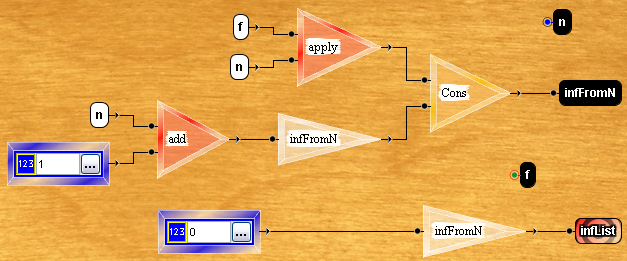
\includegraphics[scale=0.4]{Figures/gcInfList}} \quad
    \subfloat[Using the InfList() Gem To Generate Fibonacci Numbers]{\label{fig:gcInfList-b}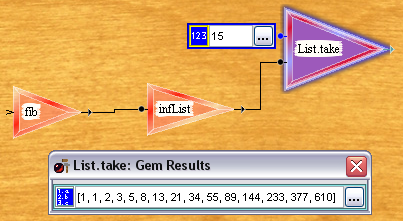
\includegraphics[scale=0.4]{Figures/gcInfListRun}}
  \end{center}
  \caption{Using The InfList() Gem}
  \label{fig:gcInfList}
\end{figure}

\subsubsection{Remedies, Workarounds, And Trade-offs}

The support for Progressive Evaluation in the Gem Cutter is quite strong.  The infinite list issue is relatively minor, only requiring one to create a new subexpression that makes use of the gem which generates the infinite list.  Perhaps a small improvement would be if the user tries to run a gem which generates an infinite list directly, to have the Gem Cutter display the evaluated results rather than just a ``out of memory'' error message.

%------------------------------------------------------------------------------------------------

\subsection{Role-Expressiveness}

As described in \sref{cgframeoutline} the dimension of Role Expressiveness tries to evaluate the environment's support for answering the user's question of ``what is this bit for?''.

\subsubsection{Discussion of Dimension}

The Gem Cutter has a number of aspects to support Role Expressiveness.  For example, all gems have meaningful identifiers attached to them (the name of the function, etc).  Modularity is supported through the use of modules and gems (functions), though while all gems from the standard libraries are organized into modules, all user-created gems go into the same module (the ``GemCutterSaveModule'' module) and creating new modules to use in the Gem Cutter is a nontrivial task (as mentioned in \sref{sec:gemCutterShortcomings}).  In terms of code ``beacons'', we found the same structures identified by Kelso in the VFPE, though rotated 90 degrees as the Gem Cutter arranges items from left to right as opposed to top down (as in the VFPE).  For example, compositional pipelines took the form of a ``vertical string of beads''\cite{Kelso02} in the VFPE, where in the Gem Cutter they became a horizontal string of Gems, etc.  In some ways, list processing created a ``staircase'' of gems, as most of the standard list processing gems (\code{map()}, \code{filter()}, \code{zip()}, etc) have two inputs, the top being a function and the bottom being a list.  A common programming idiom in the functional world is to have the output of list processing functions fed into other list processing functions, which in the case of Gem Cutter results in this left to right, rising ``staircase'' of gems.

\subsubsection{Remedies, Workarounds, And Trade-offs}

The only additional support needed for modularity in regards to the Gem Cutter is the ability for one to more easily create their own modules.  As it stands, one has to resort to writing CAL code by hand, then modifying the Gem Cutter environment to import the modules into the current workspace.

%------------------------------------------------------------------------------------------------

\subsection{Secondary Notation}

As described in \sref{cgframeoutline} the dimension of Secondary Notation explores what support the environment has for conveying extra information to users beyond the official syntax of a notation.

\subsubsection{Discussion of Dimension}

Layout in the Gem Cutter is freeform, and as such can be used to convey meaning to users.  This is very much like Prograph where layout was also freeform, and unlike the VFPE where layout was completely controlled by the environment.  Colour and visual cues are used to convey extra meaning, function gems are coloured red, user-created local functions are coloured a yellow colour, record selection gems a violet colour, and collector gems are black, and emitters are coloured white.  As well, the target gem that represents the gem's return value is coloured as a ``bullseye'' to convey the meaning that it is the overall ``target'' of the current gem.

Commenting is supported through the properties window of any collector gem or the target gem.  The Properties window for the \code{rocket1()} gem described in \sref{sec:eval:diffuseness} is shown in \fref{gcRocketProps}.  In the properties window one can describe and annotate various aspects of the gem in question.  As mentioned the same set of documentation can be done for any collector gem within a gem, thus allowing the ability to comment groups of gems.  However, individual gems other than collector gems cannot be annotated with comments.  In the case of value gems it is possible to ``name'' them by feeding a value gem into a collector gem and then naming the collector gem, however this increases the number of graphic entities on screen thereby negatively impacting Diffuseness.  Additionally, though comments are supported through the properties window of a gem, like the VFPE there is no visual cue that such a comment exists.

\insertFigure{4.5}{gcRocketProps}{The \code{rocket1()} Gem's Properties Window}

\subsubsection{Remedies, Workarounds, And Trade-offs}

The main remedy to problems associated with Secondary Notation that Green describes is to ``provide tools in the system to allow components to be labeled and described and their relationships made explicit'' \cite{green98}.  The Gem Cutter does this to a certain degree with the Properties window, but it is very coarse grained -- there is not enough support in the form of tools to allow sub-parts of gems to be documented and described.

It is also worth noting that Secondary Notation often trades off against Viscosity, as if the structure is changed, then the secondary notation becomes obsolete and also needs to be changed.  In the case of the Gem Cutter when the arguments and return types of a gem change, the properties are automatically updated, which helps to mitigate this concern.  Specifically, if arguments are removed from the gem definition, then they are also automatically removed from the properties window.  If arguments are added then an entry for the argument will be added automatically to the properties of the gem, however a meaningful description still needs to manually be added by the user.  Other metadata stored in the properties window such as author name, description of the gem, etc, will also have to be maintained manually by the user.

%------------------------------------------------------------------------------------------------

\subsection{Viscosity}

As described in \sref{cgframeoutline} the dimension of Viscosity tries to measure an environment's resistance to change.

\subsubsection{Discussion of Dimension}

The biggest issue in terms of Viscosity in the Gem Cutter is the type dependency issue between gems described in \sref{sec:gemCutterShortcomings}.  This imposes a serious impediment on a user to refactor existing gem designs.

The manual layout problem described by Kelso in \cite{Kelso02} is somewhat mitigated by the ability in Gem Cutter to instruct the environment to automatically rearrange all items on the tabletop\footnote{Via the ``Tidy Tabletop'' menu command}.  There is still overhead associated with making changes to expressions due to the having to make and break connections between gems, and move them around to make room for whatever changes need to be made.  This became particularly evident while performing the ``straw-test'' of making the small change to account for air resistance to the rocket trajectory problem, as a significant time consuming aspect of the change in the Gem Cutter version of this problem was breaking the connection between the calculation of the new horizontal and vertical velocities and the collector gem which collected these values, and inserting the gems to incorporate the change to air resistance.  In terms of time taken, incorporating the air resistance change into the Gem Cutter version of the problem was done three times, each application of the change was timed, and took 172 seconds on average to complete.  This is dramatically better than the LabVIEW (508.3 seconds) and somewhat better than the Prograph (193.6 seconds) results, but worse than the VFPE (105 seconds).

One thing worth noting is that the change for air resistance was confined only to the \code{rocket1()} gem, and not the \code{rocketTester()} gem.  Thus the type dependency issue was not encountered in this test.  If \code{rocketTester()} did have to be changed due to the changes in \code{rocket1()} the amount of time taken likely would have been dramatically higher.

\subsubsection{Remedies, Workarounds, And Trade-offs}

Green notes than an important point to consider about Viscosity is that it is not always harmful \cite{green98}.  High viscosity may encourage users to reflect more about the problem before ``diving in'' (though this would be an example of negatively impacting Premature Commitment).  Low Viscosity may encourage users to make changes more often than need be, and as a result increase the Error-Proneness of the system.

The main workaround for extremely viscous environments is to detach from the environment itself.  That is, to use a different environment with very low viscosity to plan out a solution to the problem, then to translate the solution in the low viscosity environment to the high viscosity environment.  For example, one may use pen and paper to sketch out a gem design, changing as problems are encountered, and then recreate the design in Gem Cutter.  This negatively impacts Premature Evaluation as one cannot ``execute'' a drawing on paper.  Alternatively, a possible workaround used at times by the author of this thesis was to write a solution in a textual language that was less viscous, and then translate that text-based solution to the Gem Cutter.  However, this would seem counterintuitive to the motivation behind using the Gem Cutter in the first place.

With respect to the rearranging the layout problem, a possible workaround is to heavily decompose the problem into very small functions.  Making a change to the internal structure of a gem is easy when the gem is small.  Counterbalancing this is the type dependency issue -- if another gem depends on the one being worked on then changing the type signature of the function is problematic, and the more gems there are, the greater the likelihood there will be a type dependency issue between them.

%------------------------------------------------------------------------------------------------

\subsection{Visibility}

As described in \sref{cgframeoutline} the dimension of Visibility is concerned with the environments support for making required materials easily accessible.

\subsubsection{Discussion of Dimension}

In terms of Visibility, navigational visibility is generally strong in the Gem Cutter, as the number of actions needed to find a particular gem in a gem design is usually very small, at most being a simple scrolling of the window to find what one is looking for.  If a gem's design becomes overly ``messy'' or ``cluttered'', a user can select the ``Tidy Tabletop'' option on the view menu to have the environment automatically arrange gem groupings in a top-down manner.  Alternatively, the Scope Window in the top left corner (seen in \fref{gcScopeWindow}) of the Gem Cutter interface, gives a hierarchical, tree-like listing of all components currently on the tabletop.  Clicking any item in this list will immediately center the tabletop on that item.  So in the worst case finding any item in a gem design is a matter of one or two clicks.  Note that as well, any subexpression in the Scope Window can be collapsed to allow one to focus on other parts of the gem design.  In \fref{gcScopeWindow} is seen with the ``hdist'', ``hveloc'', and ``mass'' collector gem expressions being collapsed, and all others being expanded.  

\insertFigure{2}{gcScopeWindow}{The Scope Window For The \code{rocket1()} Gem}

Predefined functions from the standard libraries are organized into modules, and are easy to find via the Gem Browser.  As well, as mentioned in \sref{sec:gemCutterUsefulApps} the Gem Browser also allows one to do a textual search for gems with particular names, input types, return types, or number of arguments.

A significant problem related to Juxtaposability in that at any given time only a single gem design can be open.  This makes working on multiple gems at the same time artificially difficult, as to open up another gem's design one has to save the current gem, then open the design of the other gem.

\subsubsection{Remedies, Workarounds, And Trade-offs}

The obvious solution to the juxtaposibility problem would be to allow multiple gems to be open at once.  Since the tabletop is a sub-window of the main Gem Cutter window, it would seem that there is no reason why this cannot take place as it would just mean allowing a second sub-window to be open.  This would allow one to switch back and forth between multiple gem designs easily.  However, given the fact that gem designs often take up a considerable amount of screen space, even if multiple gems could be open at the same time, it might be difficult or impossible to view them side-by-side.  Short of being able to ``zoom-out'' on a gem design to make it take less space (which would make seeing the individual components more difficult) it would seem that there is no solution to this problem.

As it stands, the only workaround for users to the juxtaposibility problem is to take a screenshot of a gem's design from a separate program, and then refer back to the screenshot as needed\footnote{This is what was done when doing the viscosity ``straw-test'' of making the small change to the rocket trajectory program}.  A significant limitation of this is that it is not uncommon for gem designs to scroll off the screen, making taking a screenshot of an entire gem's design difficult or impossible.

\begin{comment}

\section{Outline Of An Experiment For Evaluating The Effectiveness Of The Gem Cutter}

In the preceding section we explored a qualitative evaluation of the Gem Cutter with a bias toward a pedagogical viewpoint.  However, a useful compliment to this would be to explore a more \emph{quantitative} evaluation of the environment.  In this section we will outline an experiment which could provide a meaningful empirical evaluation of the Gem Cutter.

\subsection{Avenues of Evaluation}

\cite{Kelso02} outlined an experiment for his VFPE in which he outlined two possible avenues of for empirical evaluation of the VFPE:

\begin{enumerate}
	\item Evaluating the general adequacy of the environment
	\item Investigating Visual Programming proper
\end{enumerate}

The first is focused on conducting experiments to evaluate the general adequacy of the programming environment.  Such experiments would focus on showing quantitatively that for programmers experienced with textual languages, that the visual environment is not significantly worse than the textual alternative.  That is, that the environment is ``feature-equivalent'' to a given textual environment.

The second is for the purpose of exploring the textual/visual division.  That is, experiments designed here would be for the purpose of identifying differences that are due solely to the respective modes of display and the programming environment tools.  This was the type of experiment that Kelso outlined for his VFPE.  This requires a textual environment which is roughly equivalent to the VFPE.  
Given that the VFPE from a semantics and abstract syntax viewpoint is very similar to Haskell, Kelso believed that an experiment comparing the two would reveal differences between the visual and textual forms of representation.  Given that the Gem Cutter truly is the visual representation of CAL code, it would seem that an experiment of this form with the Gem Cutter and CAL would be more telling of the differences between the visual and the textual.

In addition to these, we can foresee other avenues for empirical evaluation of the Gem Cutter, most notably that of functional versus object-orientated programming.  There have already been studies which have explored the differences between the two paradigms (FIXME - references??), but they have largely been based solely in the textual world.  Similar experiments using the Gem Cutter (a visual environment rooted in the functional paradigm) and one of the common object-orientated environments (such as Prograph, Alice, or Scratch) would be an interesting addition to the work exploring the difference between the two paradigms.

For our purposes as educators however, we are more interested about how effective the Gem Cutter can be as a learning tool for students.  As such, we shall identify an experiment which explores two other avenues of exploration.  The first is to assess if the Gem Cutter can meet a typical set of learning objectives (ie - ``Does the student learn the concept?''), and the second assesses the transfer of skill to another environment (ie - ``Can the student apply what he/she learned to a different language?'').

\subsection{Difficulties}

Assessing which of two competing methods of instruction is more effective seems at first glance to be a simple task.  Simply teach one subject with both methods and compare the results of the two approaches.  However, as outlined by McKeachie in \cite{teachingTips} there are some difficulties or ``hidden traps'' that arise in trying to evaluate two different approaches to instruction.

The first category of problems are methodological, 

From Teaching Tips, \cite{teachingTips}:

methodological problems:

\begin{itemize}
	\item Hawthorne effect - instructor enthusiasm can influence quality of instruction, students react differently when they know they are being taught by an experimental method -- necessitates evaluation over period of time
	\item Finding control group -- different classes have different makeups of students, some instructors are better than others (so if method is successful how much is the method and how much the instructor)
\end{itemize}

criterion problem - you want to ``know what each group learned that the other did not.  Thus a comparison of the lecture method with a discussion method based on a common final examination from a textbook does not really compare what the two groups of students learned in their different classes, but rather what they learned from reading the text.''  ''criterion measure should sample progress on \textit{all} goals, not just a small sample chosen for a particular method.''  Student motivation -- students are motivated to get good grades, and thus may compensate for poor instruction, thereby obfuscating research results.

\subsection{Preparation}


\subsection{Group Selection}


\subsection{Measurement}

\section{Misc Notes}

\cite{Bayliss09} in 3.7 talks about important points in assessing the use of games, which may be relevant to this experiment.

\end{comment}